\documentclass[final]{beamer}
  \mode<presentation>
  {
% you can chose your theme here:
%  \usetheme{Aachen}
  \usetheme{I6dv}
%  \usetheme{I6pd}
%      \usetheme{Berlin}
%  \usetheme{I6pd2}
%  \usetheme{I6td}
%  \usetheme{Oldi6}
}
% \graphicspath{{figures/}}

%%%%%%%%%%%%%%%%%%%%%%%%%%%%%%%%%%%%%%%%%%%%%%%%%%%%%%%%%%%%
% PACKAGES
%%%%%%%%%%%%%%%%%%%%%%%%%%%%%%%%%%%%%%%%%%%%%%%%%%%%%%%%%%%%
\usepackage[utf8x]{inputenc}

\usepackage{amsmath,amssymb}
\usepackage[english]{babel}
\usepackage[orientation=portrait,size=a0,scale=1.6]{beamerposter}  % e.g. custom size poster
\usepackage{graphicx}

\definecolor{cpale}{rgb}{0.9,1,1}
\definecolor{gris}{rgb}{0.6,0.6,0.6}
\definecolor{violet}{rgb}{0.3, 0, 0.8}
\usepackage{tikz}
\usetikzlibrary{arrows,automata}


\newcommand{\couleur}[1]{\textcolor{violet}{#1}}
\newcommand{\coulitem}[1]{\textcolor{blue}{#1}}

\newcommand{\hytech}{\textsc{HyTech}}
\newcommand{\imitator}{\textsc{Imitator}}


% \title[Poster VALMEM]{Timed Verification of the \\[0.5cm] SPSMALL Embedded Memory}
\title[HYMITATOR]{Parametric Analysis of Hybrid Systems Using HYMITATOR \\[0.5cm]
	of Embedded Memories Using Formal Methods}


\author[Ulrich K\"uhne]{\'Etienne Andr\'e$^1$ and Ulrich K\"uhne$^2$}

\institute[LSV, LIP6 and ST]{
	$^1$LIPN, CNRS UMR 7030, Université Paris 13, France \\
	$^2$Group for Computer Architecture, University of Bremen, Germany
	}

\date{January 5th, 2010}

\begin{document}

\begin{frame}{} 

%%%%%%%%%%%%%%%%%%%%%%%%%%%%%%%%%%%%%%%%%%%%%%%%%%
%%%%%%%%%%%%%%%%%%%%%%%%%%%%%%%%%%%%%%%%%%%%%%%%%%
\begin{columns}[t]


%%%%%%%%%%%%%%%%%%%%%%%%%%%%%%%%%%%%%%%%%%%%%%%%%%
\begin{column}{.45\linewidth}
    

%-%-%-%-%-%-%-%-%-%-%-%-%-%-%-%-%-%-%-%-%-%-%-%-%-
\begin{block}{Goal}

\begin{itemize}
	\item Synthesize the timing characteristics of several embedded memory components, taking into account the electrical propagation delays through logical gates and along wires.
\end{itemize}

\end{block}
%-%-%-%-%-%-%-%-%-%-%-%-%-%-%-%-%-%-%-%-%-%-%-%-%-



%-%-%-%-%-%-%-%-%-%-%-%-%-%-%-%-%-%-%-%-%-%-%-%-%-
\begin{block}{The SPSMALL Memory}

A typical case study of the project VALMEM is the SPSMALL memory.

\begin{itemize}
	\item \coulitem{Description}
	\begin{itemize}
		\item The SPSMALL memory is a small memory with a maximum total capacity of 64\,kbits (3 to 512 words of 2 to 256\,bits).
		We first chose to model the smallest memory consisting in three words of two bits, which leads to a netlist of 305 transistors.
	\end{itemize}

% 	\begin{figure}
% 	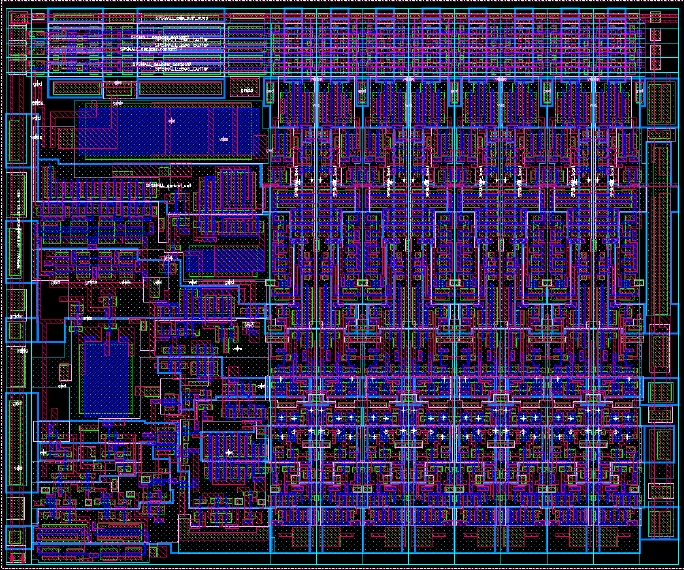
\includegraphics[width=0.5\textwidth]{spsmall_moche.jpg}
% 	\caption{Masks of SPSMALL}
% 	\end{figure}

	\item \coulitem{Description of the environment}
	\begin{itemize}
		\item The memory is  embedded into a synchronous environment: all operations (\emph{read}, \emph{write}) are synchronized with the rising edge of a unique clock (CK).
		Address (A), input data (D), write enable not (WEN) signals are latched in at the rising edge of the clock (CK).
		WEN precises the direction of a memory operation (read or write).
		Output data are internally latched at the completion of each access, and are valid until the next positive edge of CK.
		During \emph{write} operations, data written into the memory are copied back to the output data pins (write-through).
	\end{itemize}
	
% 	\begin{figure}
% 	\includegraphics[width=0.5\textwidth]{signaux_moches.jpg}
% 	\caption{Environment of SPSMALL}
% 	\end{figure}
 
	\item \coulitem{Timing description given by the datasheet}
	\begin{itemize}
		\item The datasheet given by the constructor defines the \couleur{set of timing values} corresponding to a nominal use of the memory.
		For instance, it defines the minimal clock cycle $t_{\mathit{cycle}}$.
		Moreover, two timings are defined for each input signals: the \couleur{setup timing}, $\mathit{setup}$ and the \couleur{hold timing}, $\mathit{hold}$.
		These timings define an interval around the rising edge of the clock in which the input signals have to be kept stable to be correctly interpreted by the system.
	\end{itemize}
\end{itemize}

\end{block}
%-%-%-%-%-%-%-%-%-%-%-%-%-%-%-%-%-%-%-%-%-%-%-%-%-



%-%-%-%-%-%-%-%-%-%-%-%-%-%-%-%-%-%-%-%-%-%-%-%-%-
\begin{block}{Property to be Verified}

\begin{itemize}
	\item The response timings of the memory correspond to the delay between the rising edge of the global clock, sampling an operation to be performed, and the results of the memory produced on the output pins.
	\item In particular, we aim at verifying the response time $t_{\mathit{CK}\rightarrow Q}$, corresponding to a $\mathit{write}$ operation.
	We are interested in showing that this response time $t_{\mathit{CK}\rightarrow Q}$ is smaller than the the time given by the datasheet ($\mathit{taaw}$), i.e. \couleur{$t_{\mathit{CK}\rightarrow Q} \leq \mathit{taaw}$}.
\end{itemize}

\end{block}
%-%-%-%-%-%-%-%-%-%-%-%-%-%-%-%-%-%-%-%-%-%-%-%-%-

%-%-%-%-%-%-%-%-%-%-%-%-%-%-%-%-%-%-%-%-%-%-%-%-%-
\begin{block}{Methodology}

% \begin{figure}
% \includegraphics[width=0.8\textwidth]{organisation_projet.jpg}
% \caption{The organization of the project}
% \end{figure}

\end{block}    
%-%-%-%-%-%-%-%-%-%-%-%-%-%-%-%-%-%-%-%-%-%-%-%-%-

\end{column}
%%%%%%%%%%%%%%%%%%%%%%%%%%%%%%%%%%%%%%%%%%%%%%%%%%


%%%%%%%%%%%%%%%%%%%%%%%%%%%%%%%%%%%%%%%%%%%%%%%%%%
\begin{column}{.45\linewidth}

%-%-%-%-%-%-%-%-%-%-%-%-%-%-%-%-%-%-%-%-%-%-%-%-%-
\begin{block}{From Transistors to VHDL}

\begin{itemize}
	\item \coulitem{Transistors}
	\begin{itemize}
		\item ST-Microelectronics provides the project with the description of the \couleur{transistor netlist}, with timed delays.
	\end{itemize}


		

	\item \coulitem{Functional abstraction}
	\begin{itemize}
		\item The description in transistors is automatically translated into a description in VHDL, using the tool \couleur{Mygal} developed in the framework of this project.
 		The VHDL code describes the memory under the form of a graph of functional components.
% 		Each component $i$ is associated with 2 intervals of delays: $[d^\uparrow_{i}; D^\uparrow_{i}]$ for a rising edge and $[d^\downarrow_{i}; D^\downarrow_{i}]$ for a falling edge.
	\end{itemize}

	\item \coulitem{Timed abstraction}
	\begin{itemize}
		\item The description of the delays for the transistors is automatically translated into timed intervals of delays for each gate.
	\end{itemize}

% 	\begin{figure}
% 	\includegraphics[width=0.9\textwidth]{abstraction_moche.jpg}
% 	\caption{Abstract model of the SPSMALL memory}
% 	\end{figure}

\end{itemize}

\end{block}    
%-%-%-%-%-%-%-%-%-%-%-%-%-%-%-%-%-%-%-%-%-%-%-%-%-


%-%-%-%-%-%-%-%-%-%-%-%-%-%-%-%-%-%-%-%-%-%-%-%-%-
\begin{block}{From VHDL to Timed Automata}

\begin{itemize}
	\item \coulitem{Modeling with timed automata}
	\begin{itemize}
		\item This description in gates and the delays are then automatically translated into a description in \couleur{timed automata}, an extension of finite state machines, using the tool \couleur{VHDL2TA} developed in the framework of this project.
	\end{itemize}

% %-%-%-%-%-%-%-%-%-%-%-%-%-%-%-%-%-%-%-%-%-%-%-%-%-%-%-%-%-%-%
\begin{figure}
{
\centering
\scriptsize
\begin{tikzpicture}[->, auto,node distance=5cm, thin] % semithick
  \tikzstyle{every state}=[minimum size=18pt, draw=gris, text=black, inner sep=2pt]

  \node[state, fill=cpale] (N00)               {$n_{00}$};
  \node[state, fill=cpale] (N01) [right of=N00] {$n_{01}$};
  \node[state, fill=cpale] (N10) [below of=N00] {$n_{10}$};
  \node[state, fill=cpale] (N11) [right of=N10] {$n_{11}$};

  \path
	(N00)
		edge [loop left] node {$x_4 \leq \delta_4^+$} (N00)
		edge [bend left]  node {$g_3^\uparrow$} (N10)
		edge         node {\begin{tabular}{c}
			$x_4 \geq \delta_4^-$\\
			$Q^\uparrow$\\
			\end{tabular}} (N01)

        (N01)
		edge [bend left] node {\begin{tabular}{c}
			$g_3^\uparrow$\\
			$x_4 := 0$\\
			\end{tabular}} (N11)

        (N10)
		edge [bend left]        node {\begin{tabular}{c}
			$g_3^\downarrow$\\
			$x_4 := 0$\\
			\end{tabular}} (N00)

	(N11)
		edge [loop right] node {$x_4 \leq \delta_4^+$} (N11)
		edge [bend left]  node {$g_3^\downarrow$} (N01)
		edge         node {\begin{tabular}{c}
			$x_4 \geq \delta_4^-$\\
			$Q^\downarrow$\\
			\end{tabular}} (N10)
  ;

\end{tikzpicture}

}
\caption{Example of timed automaton modeling a gate}
\label{fig:PTA-not}
\end{figure}
% %-%-%-%-%-%-%-%-%-%-%-%-%-%-%-%-%-%-%-%-%-%-%-%-%-%-%-%-%-%-%

\end{itemize}

\end{block}    
%-%-%-%-%-%-%-%-%-%-%-%-%-%-%-%-%-%-%-%-%-%-%-%-%-

%-%-%-%-%-%-%-%-%-%-%-%-%-%-%-%-%-%-%-%-%-%-%-%-%-
\begin{block}{From Timed Automata to Timing Constraints}

\begin{itemize}
	\item \coulitem{Tool \imitator{}}
	\begin{itemize}
		\item Using the tool \couleur{\imitator{}}, developed in the framework of this project, we synthesize automatically a set of symbolic linear constraints on the timings seen as parameters.
		This will allow us to \couleur{optimize the crucial timings} of the memory, such as setup and hold timing of input signals.
	\end{itemize}
\end{itemize}

\end{block}    
%-%-%-%-%-%-%-%-%-%-%-%-%-%-%-%-%-%-%-%-%-%-%-%-%-


%-%-%-%-%-%-%-%-%-%-%-%-%-%-%-%-%-%-%-%-%-%-%-%-%-
\begin{block}{References}

\begin{itemize}
	\item Remy Chevallier, Emmanuelle Encrenaz, Laurent Fribourg and Weiwen Xu.
	\coulitem{Timed Verification of a Generic Architecture of a Memory Circuit using Parametric Timed Automata}.
	International Journal of Formal Methods in System Design, vol 34(1), pp 59-81, 2009.
	
	\item \'Etienne Andr\'e, Thomas Chatain, Emmanuelle Encrenaz and Laurent Fribourg.
	\coulitem{An Inverse Method for Parametric Timed Automata}.
	International Journal of Foundations of Computer Science, vol 20(5), pp 819-836, 2009.
	
	\item \'Etienne Andr\'e.
	\coulitem{\imitator{}: A Tool for Synthesizing Constraints on Timing Bounds of Timed Automata}.
	In Martin Leucker and Carroll Morgan (eds.), ICTAC'09, LNCS 5684, pages 336-342. Springer, 2009.
\end{itemize}

\end{block}    
%-%-%-%-%-%-%-%-%-%-%-%-%-%-%-%-%-%-%-%-%-%-%-%-%-

%-%-%-%-%-%-%-%-%-%-%-%-%-%-%-%-%-%-%-%-%-%-%-%-%-
\begin{block}{The Team}

% \begin{figure}
% \includegraphics[width=0.6\textwidth]{equipe_decoupee.jpg}
% % \caption{Abstract model of the SPSMALL memory}
% \end{figure}

\end{block}    
%-%-%-%-%-%-%-%-%-%-%-%-%-%-%-%-%-%-%-%-%-%-%-%-%-

\vfill


\end{column}
%%%%%%%%%%%%%%%%%%%%%%%%%%%%%%%%%%%%%%%%%%%%%%%%%%

% \vfill

\end{columns}
%%%%%%%%%%%%%%%%%%%%%%%%%%%%%%%%%%%%%%%%%%%%%%%%%%
%%%%%%%%%%%%%%%%%%%%%%%%%%%%%%%%%%%%%%%%%%%%%%%%%%

\vfill

\end{frame}



\end{document}



%%%%%%%%%%%%%%%%%%%%%%%%%%%%%%%%%%%%%%%%%%%%%%%%%%%%%%%%%%%%%%%%%%%%%%%%%%%%%%%%%%%%%%%%%%%%%%%%%%%%
%%% Local Variables: 
%%% mode: latex
%%% TeX-PDF-mode: t
